\section{Additional Figures for Earlier Thermal Studies}
\label{app:earlierthermalfigures}
These figures retain the earlier studies' original protocols and data. Their
budgets differ from the matched-volume, fixed-power, complete-pipeline
comparison in \cref{sec:submissionstudy}; their reported speed ratios and
uncertainty summaries should not be transferred between experiments.

\begin{figure}[t]
 \centering
 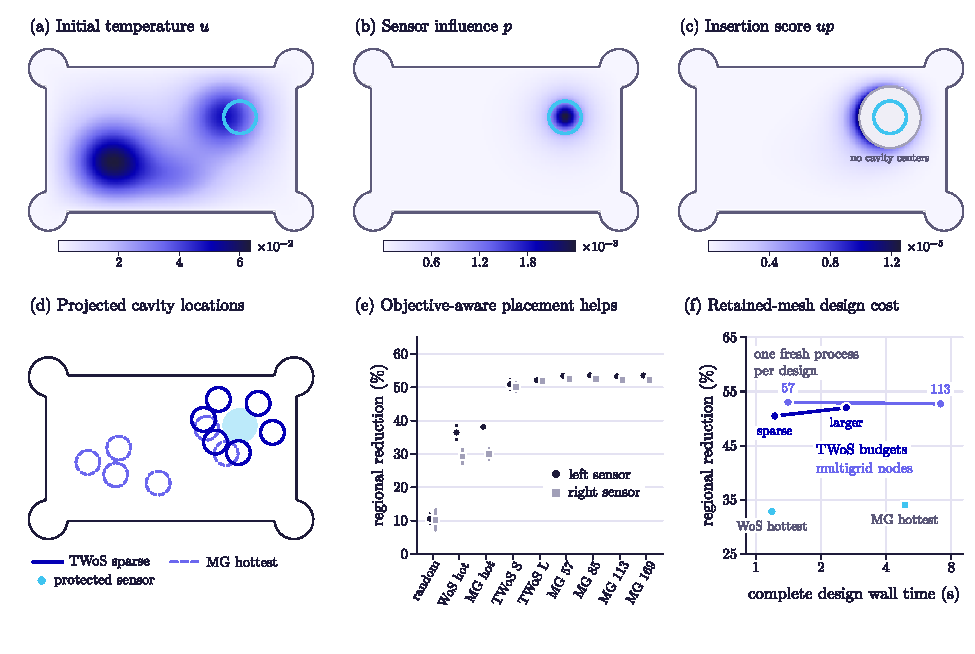
\includegraphics[width=\textwidth]{figures/distinct-adjoint-benchmark.pdf}
 \caption{Regional thermal protection with a distinct adjoint.
 (a--c) Initial temperature, sensor influence, and insertion scores on
 the same horizontal cut; each field has its own color scale.
 Cyan outlines the protected sensor; the light disk in (c) excludes
 cavity centers by the sensor radius, cavity radius, and safety gap.
 (d) Projected cavity spheres
 selected by sparse \method{} and deterministic hottest-point placement
 for the first right-sensor seed. (e) Regional temperature reductions,
 with one standard error across five complete designs. S and L denote
 the two \method{} sampling budgets. (f) Mean design quality and complete
 wall time across both sensor cases using the retained-mesh backend,
 showing both sampling budgets and the coarse/primary multigrid settings.
 The complete resolution sweep and both backend timings are in
 \cref{tab:regional}. Numerical references remain approximate;
 no finite-benefit certification is enabled in this experiment.}
 \label{fig:regional}
\end{figure}

\begin{figure}[t]
 \centering
 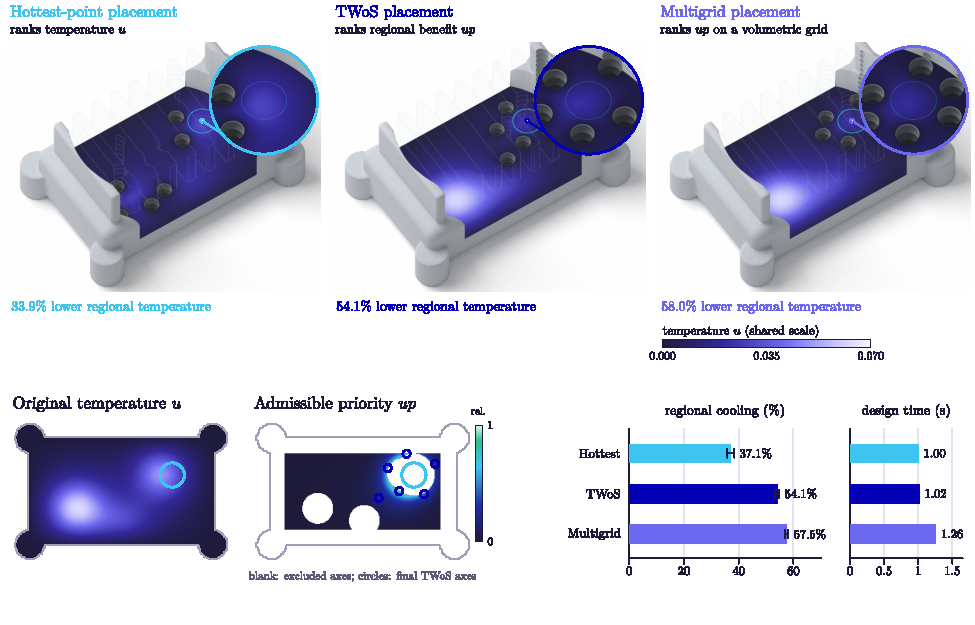
\includegraphics[width=\textwidth]{figures/accessible-channels.pdf}
 \caption{Accessible cooling with objective-aware placement.
 Top: actual saved first-seed right-sensor designs for hottest-point,
 TWoS, and coarse multigrid placement, with identical cameras, display cuts,
 lighting, and an absolute temperature scale. Magnified views show the
 protected sensor (cyan); cavity walls retain geometric shading. Faint,
 depth-tested shells indicate bars removed only for the display cut.
 The displayed cut does not enter the physical PDE. Section temperatures
 use a separate $169\times109\times85$ multigrid reference and bilinear
 display interpolation. Per-design labels use independent WoS evaluations.
 Bottom left: the original temperature and relative admissible $up$
 priority; circles mark the final TWoS axes, selected sequentially as
 fields change. Bottom right: mean cooling and complete design cost over
 both sensor positions and five seeds; error bars are one standard error
 across the five paired-seed averages. The full 50-design study, including
 random and finer-grid baselines, is in \cref{tab:accessible}.
 All methods share channel count, radius, and extent; removed volume varies.
 The point score remains a whole-channel placement heuristic, with no
 channel derivative or finite-benefit certificate asserted.}
 \label{fig:accessible}
\end{figure}

\begin{figure}[t]
 \centering
 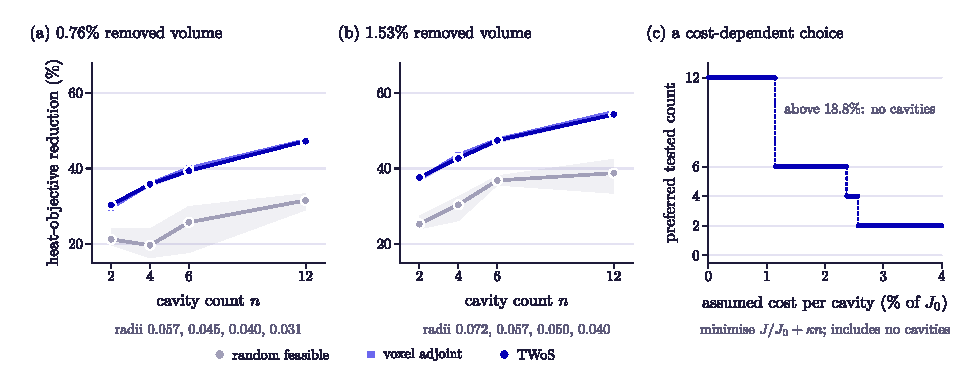
\includegraphics[width=\textwidth]{figures/bunny-budget.pdf}
 \caption{\textbf{Cavity allocation and a cost-dependent count.}
 (a--b) Cooling at two fixed removed volumes; radii are listed in count order.
 Lines are means over three complete design seeds, and shaded ranges are their
 minima and maxima, not confidence intervals. Each design is evaluated using
 four independent randomized spatial blocks with fresh WoS paths; blocks are
 shared across designs. (c) The preferred tested full-budget TWoS count after
 adding an assumed per-cavity cost to normalized compliance; the unperforated
 option is included. This is a finite-design sensitivity plot, not an estimated
 physical cost or a global optimum. All cavities have ideal cooled walls;
 at fixed volume, their total surface area increases with count.}
 \label{fig:bunnybudget}
\end{figure}

\begin{figure}[t]
 \centering
 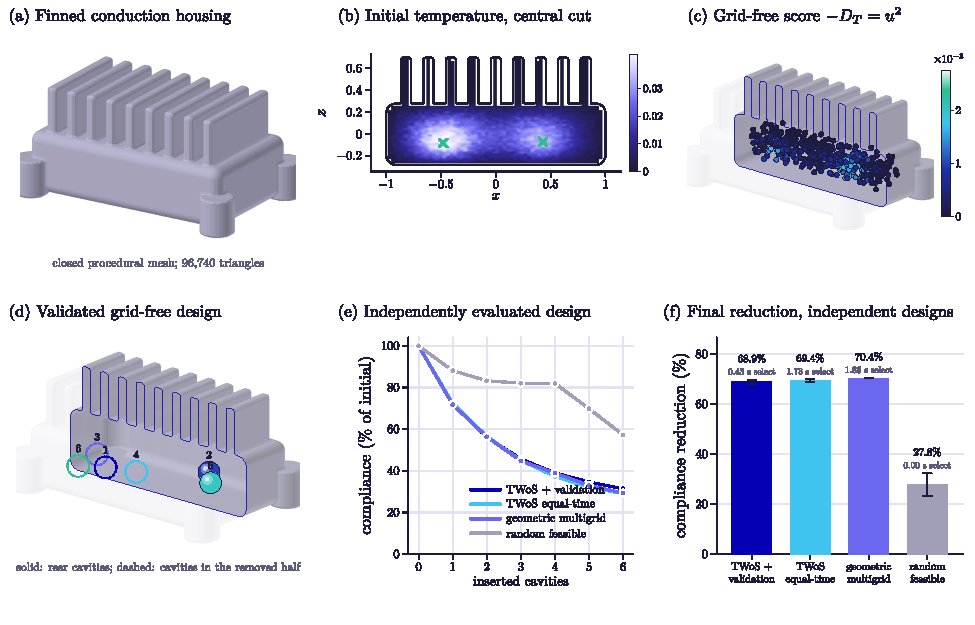
\includegraphics[width=\textwidth]{figures/engineering-housing-benchmark.pdf}
 \caption{Measured topology design on a stylized finned conduction housing.
 (a) The closed 96,740-triangle input. (b) Initial temperature on the central
 cut, with mint crosses at the two chip-source centers. (c) Direct grid-free
 topological scores inside a shaded cutaway. (d) Six cavities selected by
 scout--rank--fresh-validate; solid spheres lie in the retained half and
 dashed outlines lie in the removed half. (e) Compliance for one canonical run under
 independent reevaluation after every insertion. (f) Mean final reduction
 across five complete stochastic designs, with standard error and mean total
 selection time; multigrid uses one deterministic design and ten fresh
 objective streams. In this earlier figure, ``validation'' denotes fresh
 shortlist ranking samples; it is not the finite-benefit certificate.}
 \label{fig:housing}
\end{figure}
